\section{Evolution of Digital Identity Management}

Most digital identity issues occur because of poor reconciliation and synchronization of information (verified claims) when trust needs to be shared. This reconciliation typically involves propagating changes, reconciling differences, and mapping physical identities to their matching virtual identities. Basically there are 4 classes of Identity Management Systems.

\subsection{Centralized Identity}

At the genesis of the internet, organizations like IANA determined the validity of IP addresses in 1988, ICANN arbitrated domain names in 1998, and by 1995 certificate Authorities (CAs) stepped up to help Internet commerce sites to prove that they were who they claimed to be. [20] One common feature shared by all these organizations is that they were centralized authorities [21]. They alone had the power to determine whose identity could be trusted or not. This means that they could also deny anyone’s identity, or perform false verifications. Another problem noticed in that era was that as more and more websites were created, identities became balkanized, and users were forced to juggle multiple identities for different websites. To alleviate this problem, some organizations took a small step beyond centralization by creating hierarchies. Due to the heritable transitive nature of trust, a root Authentication agent can authorize subordinate Authentication agents to oversee their own hierarchy. However, this was not a complete solution because root Authentication agents still hold the core power of the system, just that now the power is delegated in smaller amounts to centralizations beneath them. [20] In summary a centralized Identity is characterized by administrative control by a single authority or a hierarchy [20].

\subsection{Federated Identity}

In 1999, Microsoft’s Passport initiative was one of the first to de-balkanize digital (online) identity in a new way[20]. It made it possible for users to use a single identity on multiple websites. Such an identity is called a federated identity. However, Microsoft was at the center of the federation which essentially made it almost as centralized as the traditional centralized authorities. To remedy this situation, Sun Microsoft organized the Liberty Alliance (2001) to resist the idea of centralized authorities. [20] They intend to create a true federation, however, the result was oligarchy: The power of centralized authorities was now divided amongst several powerful Authentication agents. This improved the problem of balkanization, however, each individual website remained an authority.[21] In summary, federated identity is characterized by administrative control by multiple, federated authorities.

\subsection{User-Centric Identity}

In 2000, the Augmented Social Network (ASN) designed the foundation of a new form of identity for the next generation of the internet. In their paper [22], they proposed building a “persistent online identity” into the very fabric of the internet.  After this foundation established by ASN, the Identity commons, in 2001, began to consolidate the revolution of digital identity with a focus on decentralization. They teamed up with Internet Identity Workshop (IIW) in 2005, in a series of semi-yearly meetings to advance decentralized identity. The user-centric model basically puts the user at the heart of the identity process, thus creating a better user experience. Soon this meaning was expanded to include providing the user with control over their identity and decentralized trust. Many digital identities were created through the work of the IIW, including OpenID in 2005, OpenID 2.0 in 2006, OAuth in 2010, FIDO in 2013, and OpenID Connect in 2014.[23]. As a general rule of thumb, these user-centric identities focused on user consent and interoperability. This allows a user to decide which service they want and share their identity from service to another.

It is theoretically possible for users to have full control over their identities. For example with OpenID, a user could register its own OpenID, which he can then use autonomously. Therefore, much like the federated identities, users prefer to use the OpenID from well known public websites, thus the final ownership of this identity will remain with the organizations that register them. Apart from the IIW, Facebook Connect appeared in 2008 hoping to leverage the lessons learned from OpenID. However, it allowed only the choice of provider which was Facebook, meaning that a user could connect to other websites with the Facebook Identity. This meant even more user risk with using Facebook Connect as compared to OpenID, because if Facebook for whatever reason decides to close a user account, that user also loses all identities connected with that account. The methodology seemed user-centric, but by reduction, it is really centralized Identity (where the central authority is Facebook) all over again.

In summary, a true user-centric identity is characterized by administrative control across multiple authorities without requiring a federation [20]. However, as it seems, even with the best user-centric identities more needs to be done in order to give the user full control over their identity.

\subsection{Self Sovereign Identity}

Even before the full development of the idea of self-sovereign identity, there were several hints. In 1991, Pretty Good Privacy (PGP) [24] offered the first hint of what could become a self-sovereign identity. It introduced the ’Web of Trust’ [25], which establishes trust in a peer to peer fashion with each user being an introducer or validator of a public key. This solves the political problem of who gets to validate a public key since everyone has an equal chance of validating a public key (little or no entry barrier). ’Web of Trust’ was a powerful decentralized trust management, however, it focused on email addresses, hence, it still depended on centralized hierarchies. For many reasons, PGP was not widely adopted. In 1996, Carl Ellison wrote a paper titled ”Establishing Identity Without Certification Authority” [26]. He considered PGP and centralized authorities as possible methods for defining digital identity. He settled on a protocol of repeated public key transmission and verifying the resulting identity with shared secrets over a secure channel. This allowed two parties to control their own identity without depending on the authorities. In 2000, ASN and the liberty alliance also a hint of self-sovereign identity because their developments were based on the assumption that every individual ought to have the right to control their own online identity, and for the last two decades there has also been a growing push to return identities to the people so that they could fully control them. [20] 

In general, user-centric designs turned centralized identities into interoperable federated identities with centralized control, while also respecting some level of user consent about how to share an identity. Self-sovereign identity builds on this, thus, it provides interoperable decentralized identity, however, it also provides user autonomy. It makes users the rulers of their own identity and ensures that users have the final say when it comes to their identity. The term Self-sovereign was first coined in February 2012, when developer Moxie Marlinspike wrote about ”Sovereign Source Authority” [27]. This catalyzed the work of Patrick Deegan in March that year on Open Mustard Seed, an open-source framework that gives users control of their identity. Several initiatives then started geared towards advocating for individual rights to identity. Since then Self-sovereign identity transformed from an idea to a mathematical policy, to legal policy, and now international policy especially in Europe due to the refugee crisis [All]. As the next step beyond user-centric identity, this means that apart from the user is central to the administration of identity, interoperability of a user’s identity across multiple locations (transportable), with user consent and true user control is required for user autonomy.

A Self-sovereign identity must allow ordinary users to make claims, which could include personally identifying information, group membership, or personal capability. This information may be asserted by other persons or groups. In achieving all this, it is essential to carefully protect individuals, defend against financial and privacy losses, and also prevent human rights abuses. [28] In conclusion Self-Sovereign identity is characterized by individual control across any number of authorities, providing a lifetime portable digital identity for any person, organization, or thing [20]. This identity does not depend on any centralized authority and can never be taken away because the user fully controls it.

\section{Principles of Self-Sovereign Identity}

Recent researches have made approaches towards providing self-sovereign identity, these include, ID2020 by Microsoft [29], Secure Key and IBM [30], Identity Chain [31], ERC #752 [32] [33],Estonian Identity [34], and many more. Most of these identities, with the exception of the Estonian identity use the blockchain. However, it should be noted that there is a lot more to self-sovereign identity than just decentralization. In order for an identity to be considered as self-sovereign, it must meet ten (10) principles.

\begin{enumerate}
    \item Users must exist independently of the identity.
    \item Users must be able to control their identities, thus be the ultimate authority on their own identity.
    \item Users must have access to their own data within their identity.
    \item All systems and algorithms regarding the identity must be transparent.
    \item Identities must be persistent, preferably last a lifetime, or for as long as the user wishes
    \item Identities must be easily transportable, thus must not be held by a single third-party (entity). 
    \item Identities must be as widely usable as possible (interoperability).
    \item Users must be given the chance to consent to the use of their identity. 
    \item Disclosure of claims must be minimized (minimization), thus, when identity data is used, only the minimum amount necessary to achieve the required task must be exposed.
    \item In cases of conflict, the rights of the user must be protected.
\end{enumerate}

In the light of the above, it is crystal clear the evolution of identities right from centralized identities have gravitated towards self-sovereign (more decentralized) identities. Self-sovereign identities are the state of the art today in Digital Identity Management systems.

\section{The BlockChain}

Blockchain technology has become popular since the introduction of bitcoin as a digital currency. The bitcoin mechanism was introduced by Satoshi Nakamoto in 2008 in a paper entitled Bitcoin: A Peer-To-Peer Electronic Cash System [4]. that was the reason blockchain came to the community. the technical concept is blockchain is something like a database but different functionalities.  A distributed network is necessary for the blockchain and there is a ledger that publicly available for everyone [35].

\begin{figure}[H]
    \centering
    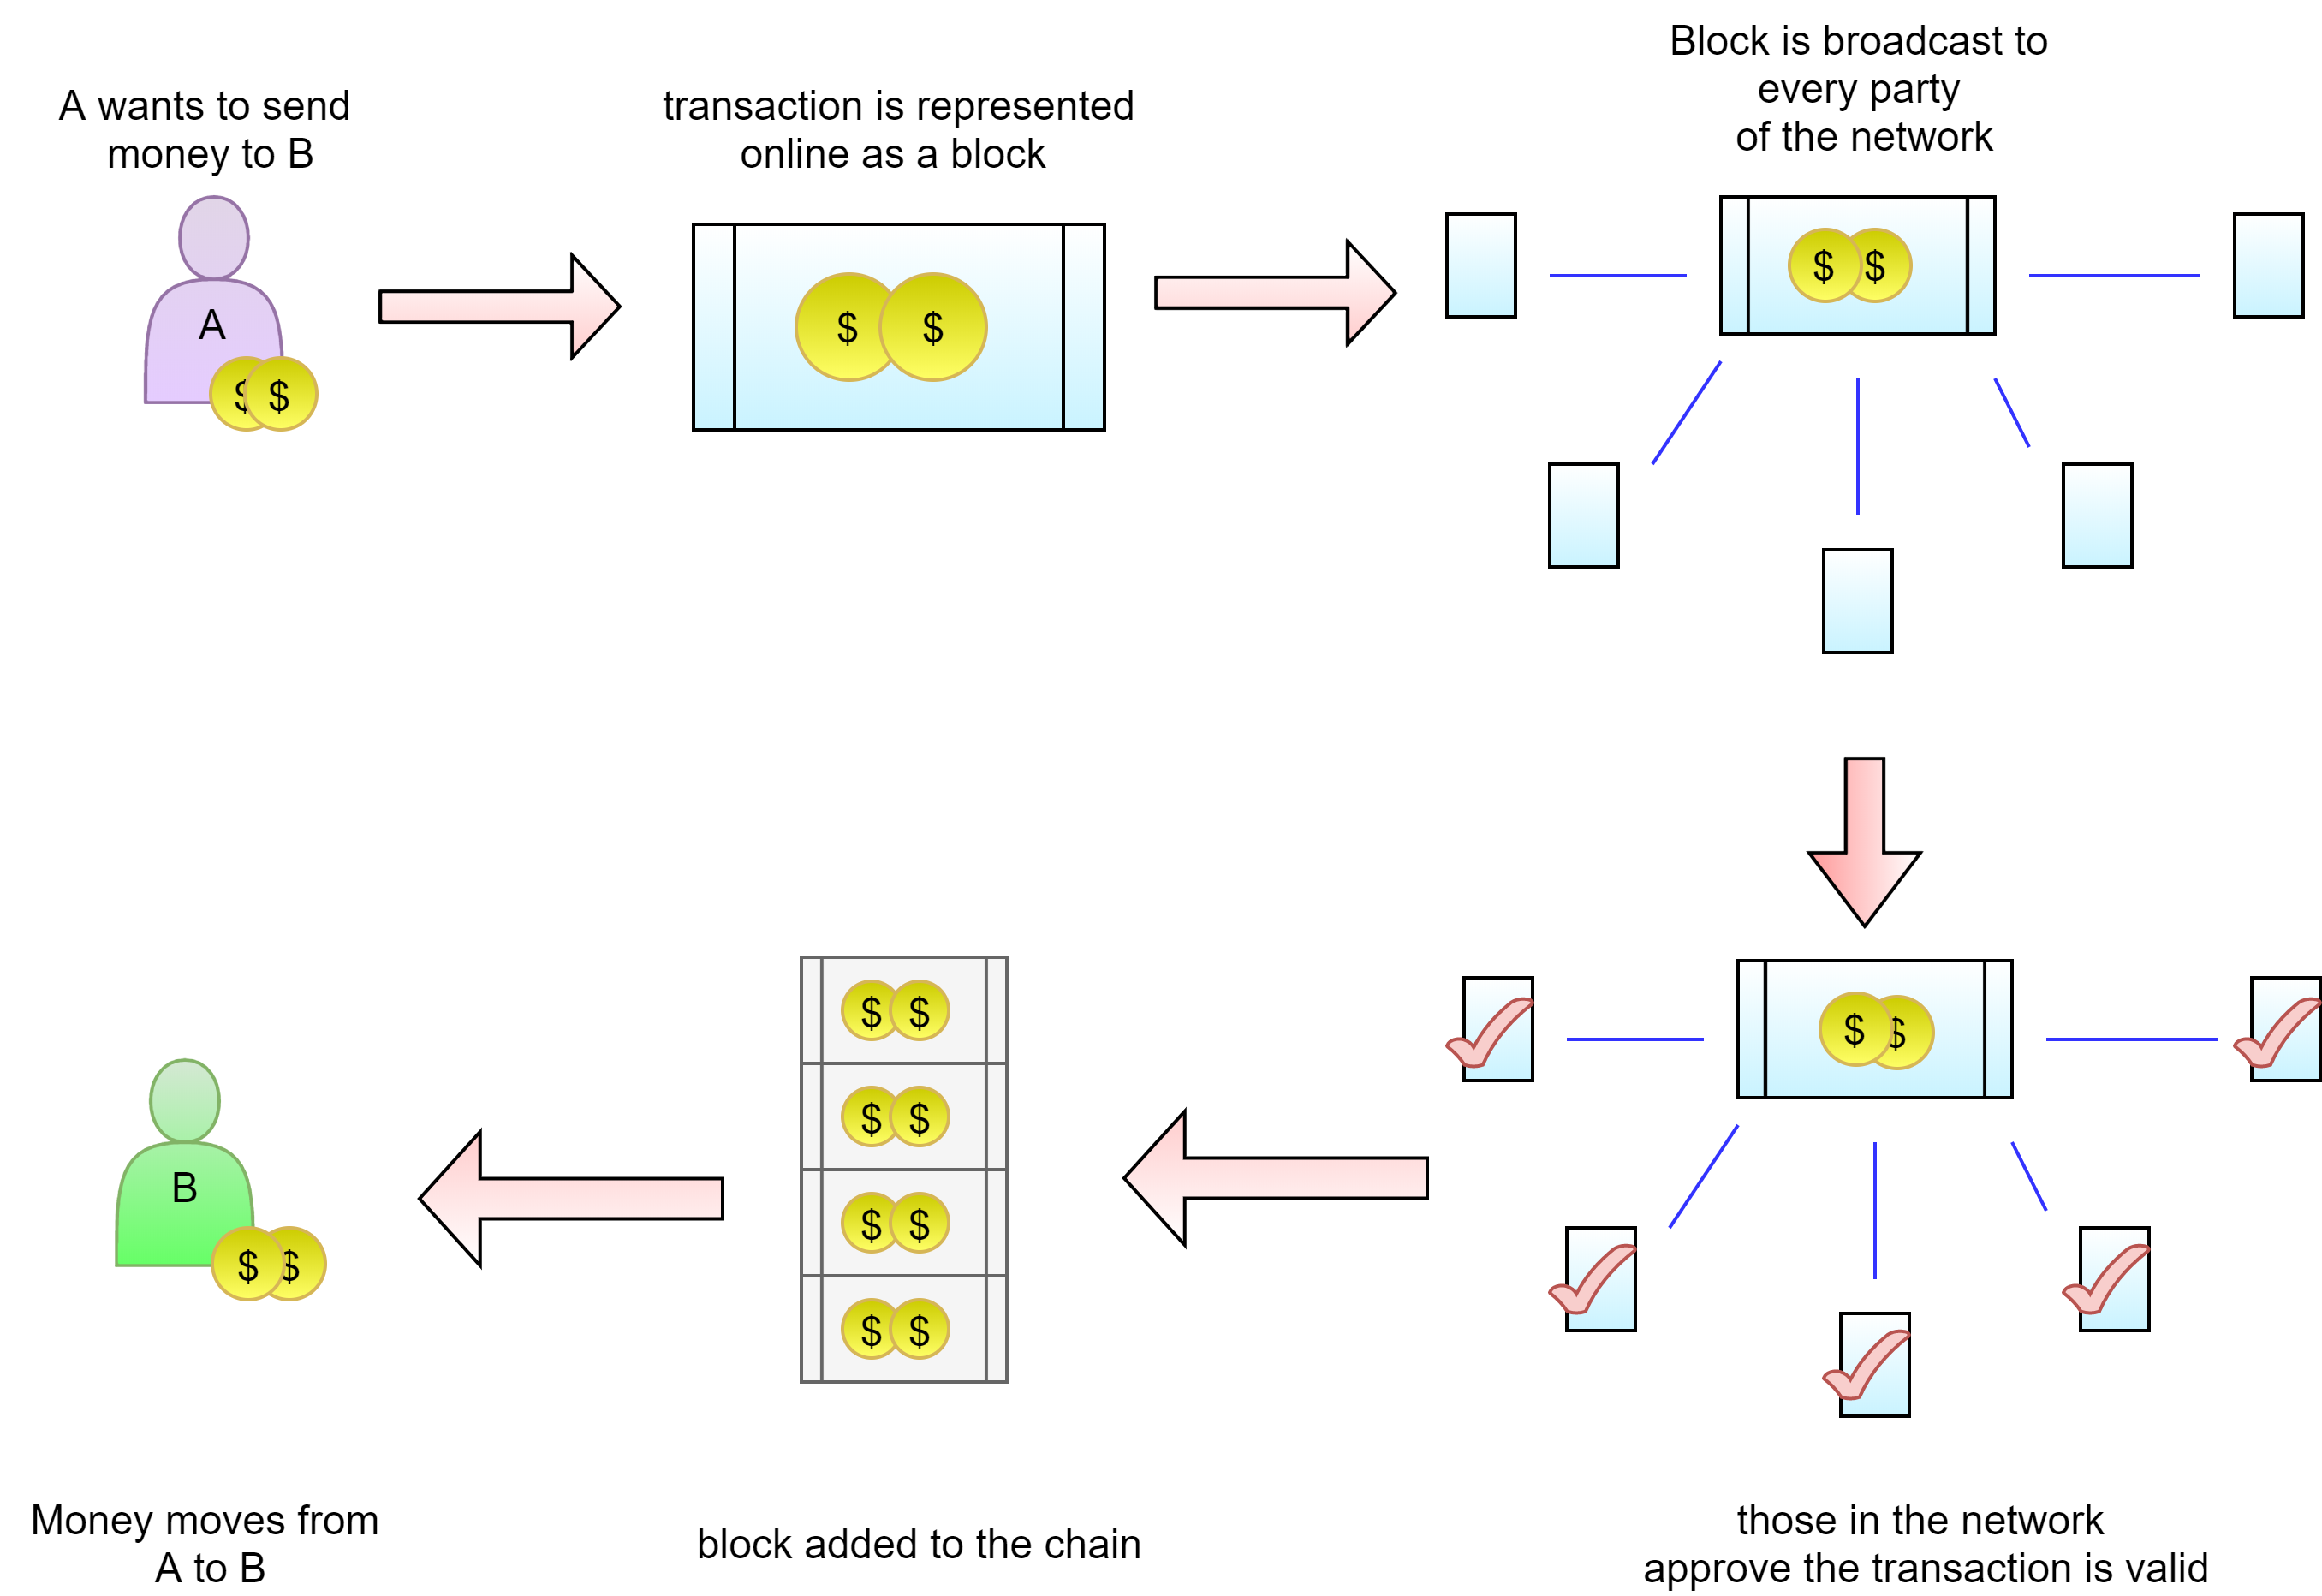
\includegraphics[scale=0.3]{6.png}
    \caption{blockchain architecture}
    \label{fig:threshold}
  \end{figure}

  
  Blockchain has two fundamental features. The blockchain is public.  Blockchain is also encrypted since it uses encryption involving public and private keys to guarantee its security. Figure xx represents the general idea of how this technology works, referring to its application for bitcoin. The bitcoin system orders transactions by placing them in groups called blocks and then linking these blocks through what is called a blockchain. These blocks are linked to each other (like a chain) in a linear, chronological order, with every block containing the hash of the previous block. Furthermore, as blockchain establishes the new era of the digital economy, there are seven design principles for creating software, services, business models, markets, organizations, and even governments on the blockchain [36]. These are detailed below. 

  \subsection{Networked integrity}

  The system lets the network reach a consensus (the acceptance and verification by all the users in the network) algorithmically on what happened and record it cryptographically on the blockchain.  Each block should guarantee that the next block is validated. all transactions are public, and it leads to a traceable mode of transactions

  \subsection{Distributed power}

  there is no single point of failure because the network is distributed. If a central authority manages to blackout or cuts off an individual or group, the system will still survive. Everyone can see what is happening if some of the networks attempt to overwhelm the whole.

  \subsection{Value as incentive}

  Imagine a peer-to-peer network of solar panels for which the homeowner receives real-time compensation on the blockchain for generating sustainable energy.

  \subsection{Security}

  Anyone who wants to participate must use cryptography. In Satoshi’s paper, he claimed that participants were required to use a public key infrastructure (PKI) for establishing a secure platform. The PKI is an advanced form of asymmetric cryptography, in which the user receives two keys that do not perform the same function: one is for encryption and the other for decryption.

  \subsection{Privacy}

  Individuals control their own data, not a single party. On a blockchain, participants can choose to maintain any degree of personal anonymity in the sense that they do not need to attach any personal details to their identity or store those details in a central database. Additionally, the identification and verification layer are separate from the transaction layer.

  \subsection{Rights preserved}
  Ownership rights are transparent and enforceable. Individual freedoms are recognized and respected. As a ledger of everything, the blockchain can serve as a public registry. through a tool called Proof of Existence (PoE), a site that creates and registers cryptographic digests of deeds, titles, receipts, or licenses on the blockchain. The hash of the document is calculated on the user’s machine, not on the PoE site, thus ensuring the confidentiality of the content.

  \subsection{Inclusion}
  there is no barriers because blockchain let everyone to join it. so the economy becomes wider. Even if the first blockchain was run through the internet, it can be run through without the internet.  the simple way of payment verification was introduced through this. This would majorly lower the cost of transmitting funds.

  \section{Why Identity Management Matches Blockchain}

  BlockChain by design is decentralized, thus, it provides a centralized approach to Identity Management. In most state of the art systems, users store their identity in their personal decentralized wallets thus eliminating the problems of centralization. This decentralization also provides a large degree of mobility and user control to such identities. A blockchain Identity also automatically provides a clear separation between the roles of Authentication agents and Authorization agents, hence degrading the probability of collision of these agents against a Subject. In most cases Authentication and Authorization agents may be completely decoupled, thus removing the incentive to misappropriate Subject data. Lastly, trust scales very well in the BlockChain environment as compared to traditional central server solutions. This is simply because new entrants into the BlockChain Identity only need to trust the consensus algorithm as compared to trusting a server or even a group of servers.

